\subsection{Testing for HTTP Parameter pollution - OTG-INPVAL-004}
\subsubsection{BANK-APP}
\begin{tabular*}{\textwidth}{ p{.20\textwidth} | p{.75\textwidth} }\hline
    & \textbf{BANK-APP} \\ \hline
    \textbf{Observation} & GET and POST request always interpreted the last parameter if the parameter was specified twice or more times. Furthermore, it could be observed that specifying another ID for \code{http://IP\_ADDRESS/secure-coding/public/view\_transaction.\allowbreak php?id=ID} while logged in as a client, shows the transaction even if it does not belong the the client. \\
    \textbf{Discovery} & With ZAP GET and POST requests were modified and parameters were specified more than once to see how the application interprets the request. The results were that if a parameter was specified twice or more times, the last occurrence was interpreted. \\
    \textbf{Likelihood} & Changing GET and POST parameters is not difficult. \\
    \textbf{Impact} & The vulnerability is that specifying another transaction ID reveals the transaction as long as it exists. Gaining access to transactions not belonging to the account is a confidentiality breach. \\
    \textbf{CVSS} &
        \begin{tabular}{l | l}
            Attack Vector           & \textcolor{red}{Network} \\
            Attack Complexity       & \textcolor{red}{Low} \\
            Privileges Required     & \textcolor{BurntOrange}{Low} \\
            User Interaction        & \textcolor{red}{None} \\
            Scope                   & \textcolor{Green}{Unchanged} \\
            Confidentiality Impact  & \textcolor{red}{High} \\
            Integrity Impact        & \textcolor{Green}{None} \\
            Availability Impact     & \textcolor{Green}{None}
        \end{tabular}
    \\ \hline
\end{tabular*}

\subsubsection{SecureBank}
\begin{tabular*}{\textwidth}{ p{.20\textwidth} | p{.75\textwidth} }\hline
    & \textbf{SecureBank} \\ \hline
    \textbf{Observation} & POST request always interpreted the last parameter if the parameter was specified twice or more times. Viewing account related information does not depend on POST or GET requests. \\
    \textbf{Discovery} & With ZAP POST requests were modified and parameters were specified more than once to see how the application interprets the request. The results were that if a parameter was specified twice or more times, the last occurrence was interpreted. Account related information is not specified over GET or POST requests. \\
    \textbf{Likelihood} & N/A \\
    \textbf{Impact} & N/A \\
    \textbf{CVSS} & N/A \\ \hline
\end{tabular*}

\subsubsection{Comparison}
Since simply specifying another transaction ID in the GET parameter in BANK-APP can reveal transactions, which do not belong to the user account, it is a high confidentiality breach. SecureBank is immune regarding HTTP parameter pollution. Figure~\ref{fig:trans_pollut} shows an example for gaining access to a transaction which does not belong to the client.

\begin{figure}[ht]
	\centering
	\begin{subfigure}{.8\textwidth}
		\centering
		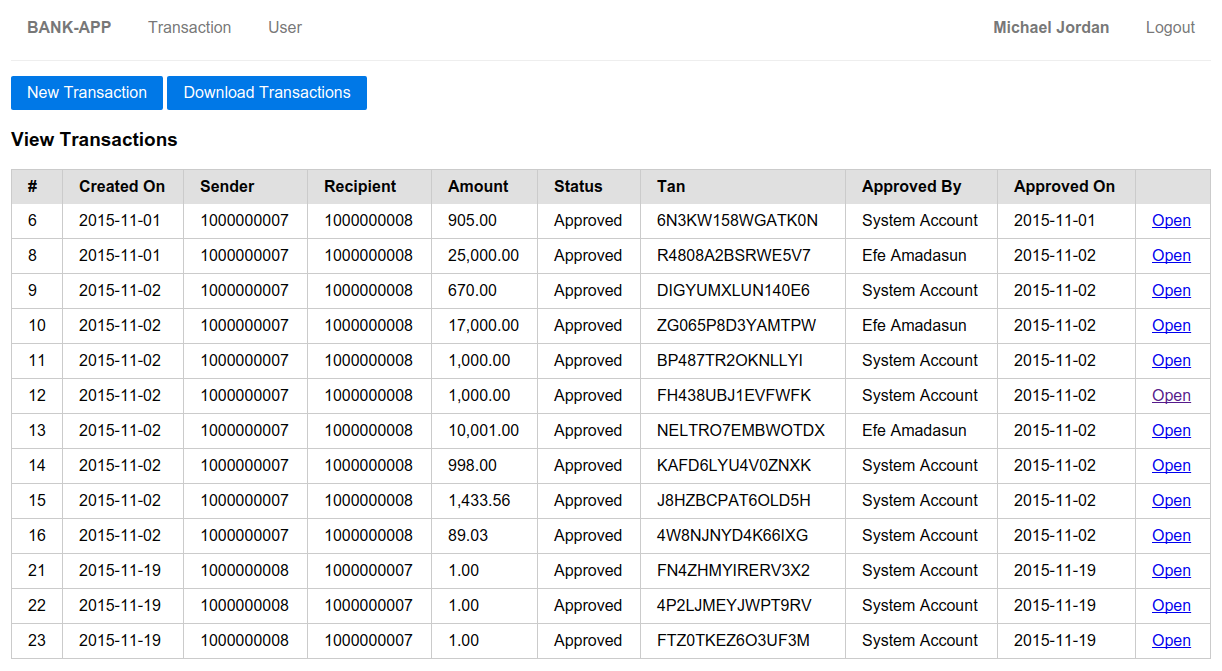
\includegraphics[width=\linewidth]{figures/OTG-INPVAL-004_1.png}
		\caption{Client transaction overview}
	\end{subfigure}
	\begin{subfigure}{.8\textwidth}
		\centering
		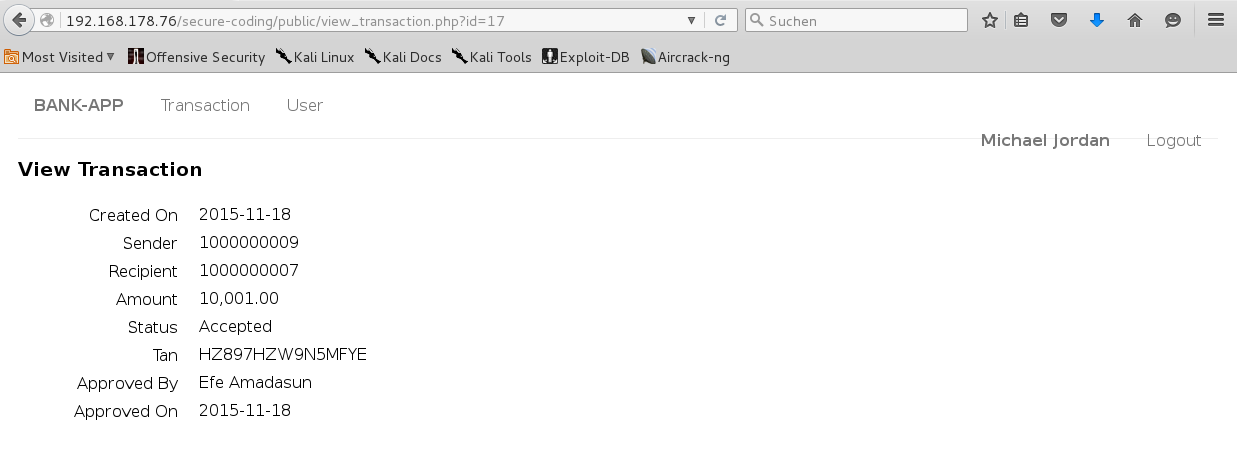
\includegraphics[width=\linewidth]{figures/OTG-INPVAL-004_2.png}
		\caption{Transaction with ID 17, which was not visible in transaction overview}
	\end{subfigure}
	\caption{BANK-APP HTTP parameter pollution: client can view transaction, which does not belong to his/her account}
	\label{fig:trans_pollut}
\end{figure}

\clearpage